\section{Ensemble Learning}

\subsection{Random Forests}

\begin{figure}[h]
    \begin{lstlisting}[gobble=8]
        for b = 1 to B:
            Retrieve a bootstrap sample
            Grow a full decision tree on the sample with random features
        return ensemble 
    \end{lstlisting}
    \caption{Random Forest construction process}
\end{figure}

\begin{align*}
    f(x) &= \frac{1}{B}\sum^{B}_{b=1} T_b(x) & \text{[Regression]}\\
    f(x) &= \text{majority vote} \{T_b(x)\}^{B}_{1} & \text{[Classification]}\\
\end{align*}

\subsection{Gradient Boosted Trees}

\begin{figure}[h]
    \begin{lstlisting}[gobble=8]
        fit tree to data
        calculate gradient

        while loss not acceptable:
            fit new tree to negative gradient
    \end{lstlisting}
\end{figure}

\begin{align*}
    s(x_i) &= \frac{e^{x_i}}{\sum^K_{k=1} e^{x_k}} & \text{[Softmax Function]}\\
    L_{\text{CE}} (y, \hat{y}) &= -\sum^K_{k=1} y \log \hat{y}& \text{[Cross Entropy Loss]}\\
    f(x) &= f(x) - \alpha \frac{\partial L(y, f(x))}{\partial f(x)} & \text{[Model update]}\\
    &= f(x) - \alpha \left[s(f(x)) - y\right]&\\
\end{align*}

\begin{figure}[h]
    \centering
    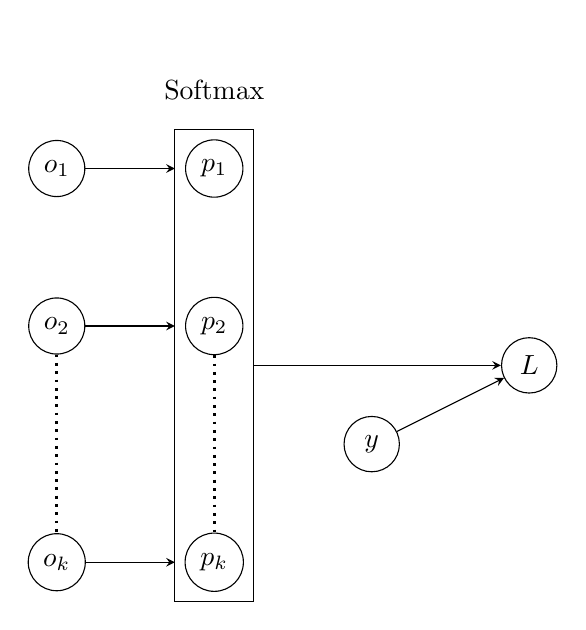
\begin{tikzpicture}[
        node/.style=draw, circle, minimum width=2em,
        forward/.style=->, >=stealth,
        scale=2
    ]
        \node[node] (o1) at (0, 0) {$o_1$};
        \node[node] (o2) at (0, -1) {$o_2$};
        \node[node] (ok) at (0, -2.5) {$o_k$};
        \draw[dotted, line width=1pt] (o2) -- (ok);
        \node[node] (p1) at (1, 0) {$p_1$};
        \node[node] (p2) at (1, -1) {$p_2$};
        \node[node] (pk) at (1, -2.5) {$p_k$};
        \draw[dotted, line width=1pt] (p2) -- (pk);
        \node[] (sm) at (1, 0.5) {Softmax};
        \draw (0.75, 0.25) rectangle (1.25, -2.75);
        \node[node] (y) at (2, -1.75) {$y$};
        \node[node] (l) at (3, -1.25) {$L$};
        \draw[forward] (o1) -- (0.75, 0);
        \draw[forward] (o2) -- (0.75, -1);
        \draw[forward] (ok) -- (0.75, -2.5);
        \draw[forward] (y) -- (l);
        \draw[forward] (1.25, -1.25) -- (l);
    \end{tikzpicture}
    \caption{Softmax computation graph for gradient boosted tree output}
\end{figure}


\subsubsection{Derivations}
Derivative of softmax output $p_j$ with respect to single $f(x)$ output $o_i$ to:\\
\begin{align*}
    \frac{\partial p_j}{\partial o_j} &= \frac{\partial}{\partial o_i} \frac{e^{o_j}}{\sum^K_{k=1} e^{o_k}} \\
    &= \frac{ (\frac{\partial}{\partial o_i} e^{o_j})(\sum^K_{k=1} e^{o_k}) - (e^{o_j})(\frac{\partial}{\partial o_i} \sum^K_{k=1} e^{o_k}) }{ (\sum^K_{k=1} e^{o_k})^2 }\\
    &= \begin{cases} i = j & \frac{ e^{o_j} \sum^K_{k=1}e^{o_k} - (e^{o_j})^2 }{ (\sum^K_{k=1}e^{o_k})^2 }\\ i \neq j & \frac{ 0 - e^{o_j}e^{o_i} }{ (\sum^K_{k=1}e^{o_k})^2 }\\ \end{cases}\\
    &= \begin{cases} i = j & p_j - p_j^2\\ i \neq j & -p_jp_i\\ \end{cases}\\
\end{align*}

Derivative of loss $L$ with with respect to single $f(x)$ output $o_i$ to:\\
\begin{align*}
    \frac{\partial L}{\partial o_i} &= \frac{\partial}{\partial o_i} \left[- \sum^K_{k=1} y_k \log p_k \right]\\
    &= - \left[\sum^K_{k=1} \frac{\partial}{\partial o_i} y_k \log p_k \right]\\
    &= - \left[\sum^K_{k=1} \frac{y_k}{p_k} \frac{\partial}{\partial o_i}  p_k \right]\\
    &= - \left[ \frac{y_i (p_i - p_i^2)}{p_i} + \sum^K_{k\neq i} \frac{-y_k(p_kp_i)}{p_k} \right]\\
    &= - \left[ y_i (1-p_i) - \sum^K_{k\neq i} y_k p_i \right]\\
    &= - \left[ y_i - p_iy_i - p_i\sum^K_{k\neq i} y_k \right]\\
    &= - \left[ y_i - p_i\sum^K_{k=1} y_k \right]\\
    &= - \left[ y_i - p_i \right]\\
    &=  p_i - y_i\\
\end{align*}

\textbf{Resources}
\begin{enumerate}
    \item Artificial Intelligence: A Modern Approach~\cite{russell1}
    \item The Softmax function and its derivative~\cite{bendersky1}
    \item Gradient Boosting Machine (GBM)~\cite{liu1}
\end{enumerate}
